\paragraph{}
	  A l'\`ere de l'information, la cyber-sécurité est un défi omniprésent. Les attaques peuvent cibler n'importe quel site Internet pour un nombre croissant de raisons. Un manque de sécurité dans une application peut causer des dysfonctionnements, des arrêts complets de service ainsi que des pertes de données dommageables pour les utilisateurs et l'image de l'entreprise. Pour s'en prémunir, les entreprises doivent mettre en place des mesures de sécurité strictes dans le processus de développement de leur applications Web. \\
	  Cette section expose quelques failles de s\'ecurit\'e li\'ees aux applications web et quelques bonnes pratiques pour y rem\'edier.
	  
	\subsection{Notion de hacker et de cracker}
	  \paragraph{}
	    Un hacker est une personne qui, par jeu, goût du défi ou souci de notoriété, cherche à contourner les protections d'un logiciel, à s'introduire frauduleusement dans un système ou un réseau informatique \cite{A} \footnote{Recommandation officielle : fouineur.}.\\Un cracker, quant à lui, s’introduit tout aussi frauduleusement dans un système informatique pour en entraver ou en fausser le fonctionnement. Son action est souvent plus dévastatrice.
		

	\subsection{Mode opératoire d'une attaque informatique}
	  \paragraph{}
	    Une attaque informatique peut être décomposée en une suite d’étapes ou phases. Lorsqu’elles sont réunies, ces étapes forment une méthodologie complète pour mener à bien une attaque informatique. L’établissement d’une méthodologie permet de décomposer une procédure complexe en une suite de tâches gérables de taille plus réduite. Ainsi nous regroupons cette méthodologie en quatre étapes qui sont \textbf{la reconnaissance}, \textbf{les scans}, \textbf{l'exploitation}, \textbf{la post-exploitation et le maintien d'accès} \footnote{La post exploitation et le maintien d'accès forment une étape.}\cite{c}.
	      
	  \subsubsection{La reconnaissance}
	    \paragraph{}
	      La reconnaissance, ou recueil d’informations, est probablement la plus importante des quatre phases. Plus le hacker passe du temps à collecter des informations sur sa cible, plus les phases suivantes auront une chance de réussir\cite{c}. En effet la reconnaissance permet de connaitre la cible dans les détails, de connaître les points forts et surtout les points faibles afin de notifier les prochaines possibilités d'attaque.

	  \subsubsection{Les scans}
	    \paragraph{}
	      Les scans sont des procédés ayant pour objectif d’identifier les systèmes actifs et les services qui existent sur les systèmes scannés. Dans ce cadre, le hacker prend le soin de vérifier l'activité d'un système, de trouver les portes ouvertes (les ports), de vérifier les processus tournant sur le système et d'aller à la recherche des vulnérabilités. Ce stade requiert une compréhension plus avancée des systèmes informatiques pour mieux comprendre les résultats recueillis \footnote{Informations recueillies au cours du scan}\cite{c}.
	      
	  \subsubsection{L'exploitation}
	    \paragraph{}
	      En termes simples, l’exploitation consiste à obtenir un contrôle sur un système. Toutefois, il est à notifier que tout exploit ne conduit pas à la compromission intégrale d’un système. Un hacker peut se servir donc d'un exploit pour télécharger des contenus dont il ne détient pas la propriété pendant qu'un autre utilise un exploit pour crypter les fichiers du système. L'utilisation de l'un des exploits \footnote{Un exploit est le moyen par lequel un attaquant, ou un pentester en l’occurrence, profite d’un défaut dans un système, une application ou un service.} dépend donc de l'objectif visé par le hacker \cite{E}.

	  \subsubsection{Post exploitation et maintien d’accès}
	    \paragraph{}
	      Cette étape consiste à couvrir les traces de l'intrus agissant afin de ne pas se faire repérer \cite{E}. Il permet aussi à ce dernier de faciliter ses prochains accès à la machine victime par l'installation de portes dérobées communément appelées "Backdoor". Ainsi, il n'aura plus besoin de reprendre toutes les étapes de son processus pour accéder à la machine dont il a eu \`a prendre le contrôle.\\ \\
	      

	\begin{figure}[H]
	  \begin{center}
	    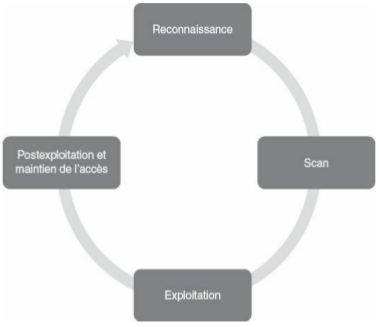
\includegraphics[scale=0.5]{images/zeh_cycle.png}
	  \end{center}
	  \caption[Représentation cyclique de la méthodologie ZEH.]
	    {Méthodologie ZEH, Patrcick Engebretson, "Les bases du hacking", PEARSON 2013}
	    \label{Methodologie d'intrusion}
	\end{figure}


	\paragraph{}
	  La méthodologie d'attaque étant cernée, nous allons maintenant présenter les différentes failles auxquelles sont expos\'ees les applications web.	    
			    

	\subsection{Menaces et risques applicatifs}
	  \subsubsection{Failles de Sécurité}
	    \paragraph{}
	    Le projet Open Web Application Security Project (\gls{owasp}) est une communauté ouverte destinée à permettre aux organisations de développer, d'acheter et de gérer des applications et des API fiables. Tous les outils, documents, vidéos, présentations et chapitres OWASP sont gratuits et ouverts à toute personne intéressée par l'amélioration de la sécurité des applications. L'approche de la sécurité des applications en tant que problème de personnes, de processus et de technologie est  préconis\'ee, car les approches les plus efficaces en matière de sécurité des applications nécessitent des améliorations dans ces domaines. OWASP produit aussi de nombreux types de matériaux de manière collaborative, transparente et ouverte. Le projet soutient la recherche innovante en matière de sécurité avec des subventions et des infrastructures.
	    
	    \paragraph{}
	    L'OWASP Top 10 est un document de sensibilisation puissant pour la sécurité des applications Web. Il représente un large consensus sur les risques de sécurité les plus critiques pour les applications Web. Les membres du projet incluent une variété d'experts en sécurité du monde entier qui ont partagé leur expertise pour produire cette liste.
	    Nous recommandons \`a toutes les entreprises d'adopter ce document de sensibilisation au sein de leur organisation et de commencer à faire en sorte que leurs applications Web minimisent ces risques. L'adoption du Top 10 de l'OWASP est peut-être la première étape la plus efficace pour changer la culture de développement de logiciels au sein de votre organisation en une culture qui produit du code sécurisé.
	    \paragraph{}
	    Cette mise à jour majeure (celle de 2017) ajoute plusieurs nouveaux problèmes, dont deux problèmes sélectionnés par la communauté - \textbf{A8: 2017 - Dés\'erialisation non sécurisée} et \textbf{A10: 2017 - Insuffisance de Logs et de Surveillance}. Les deux principales différences par rapport aux versions précédentes du Top 10 d'OWASP sont les retours substantiels de la communauté et les données complètes rassemblées par des dizaines d'organisations, probablement la plus grande quantité de données jamais rassemblées dans la préparation d'une norme de sécurité applicative. Cela nous permet de croire que le nouveau Top 10 d'OWASP aborde les risques de sécurité applicative les plus importants auxquels sont confrontées les entreprises.
	    \paragraph{}
	    L'un des principaux objectifs du Top 10 d'OWASP est d'éduquer les développeurs, les concepteurs, les architectes, les gestionnaires et les organisations sur les conséquences des faiblesses les plus courantes et les plus importantes de la sécurité des applications Web. Le Top 10 fournit des techniques de base pour se protéger contre ces zones problématiques à haut risque et fournit des indications sur les endroits où aller.
	    \paragraph{}
	    Les attaquants peuvent potentiellement utiliser de nombreux chemins différents à travers votre application pour nuire à votre entreprise ou organisation. Chacun de ces chemins représente un risque qui peut ou non être suffisamment sérieux pour justifier une attention. Parfois, ces chemins sont triviaux à trouver et à exploiter, et parfois ils sont extrêmement difficiles. De même, le préjudice causé peut être sans conséquence, ou vous mettre à la faillite. Pour déterminer le risque pour votre organisation, vous pouvez évaluer la probabilité associée à chaque agent de menace, vecteur d'attaque et faiblesse de la sécurité et le combiner avec une estimation de l'impact technique et commercial sur votre organisation. Ensemble, ces facteurs déterminent votre risque global.
	    
	    \subsubsection{OWASP Top 10 - 2017}
	      \paragraph{}
	      Le rapport « OWASP Top 10 » permet ainsi à l’équipe projet de se focaliser sur la protection de l’application Web
	      face aux menaces les plus importantes, ce qui est moins co\^uteux et plus facilement réalisable
	      que d’essayer de se protéger de tous les dangers. L’OWASP établit le classement 2017
	      ci-dessous, dont chacune des failles est développée dans les sous-sections suivantes :
	            
	  \begin{enumerate}[label=\roman*)]
		\vspace*{0.8cm} \item \textbf{Injection} \vspace*{-0.4cm}
		\paragraph{}
		Des erreurs d'injection, telles que l'injection \gls{sql}, \gls{nosql}, se produisent lorsque des données non fiables sont envoyées à un interpréteur dans le cadre d'une commande ou d'une requête. Les données hostiles de l'attaquant peuvent amener l'interpréteur à exécuter des commandes inattendues ou à accéder aux données sans autorisation appropriée.
		\paragraph{}L'injection peut parfois conduire à une prise en charge complète de l'hôte. L'impact métier dépend des besoins de l'application et des données.
		\paragraph{}La prévention de l'injection nécessite de séparer les données des commandes et des requêtes. L'option préférée consiste à utiliser une \gls{api} sécurisée, qui évite l'utilisation complète de l'interpréteur ou fournit une interface paramétrée, ou migre pour utiliser les outils \gls{orm} (Object Relational Mapping Tools)

		\vspace*{0.8cm} \item \textbf{Authentification brisée} \vspace*{-0.4cm}
		\paragraph{}
		L'authentification brisée est g\'en\'eralement connue en anglais sous le nom de \textbf{Broken Authentication}.
		Les fonctions d'application liées à l'authentification et à la gestion de session sont souvent incorrectement implémentées, permettant aux pirates de compromettre les mots de passe, clés ou jetons de session ou d'exploiter d'autres failles d'implémentation pour prendre temporairement ou définitivement les identités des autres utilisateurs. La prévalence de l'authentification brisée est généralisée en raison de la conception et de la mise en œuvre de la plupart des contrôles d'identité et d'accès. La gestion de session est le fondement des contrôles d'authentification et d'accès et est présente dans toutes les applications avec état.
		\paragraph{}
		Les attaquants doivent avoir accès à seulement quelques comptes ou à un seul compte administrateur pour compromettre le système. Selon le domaine de l'application, cela peut permettre le blanchiment d'argent, la fraude à la sécurité sociale et le vol d'identité, ou divulguer des informations hautement sensibles protégées par la loi.
		\paragraph{}
		Lorsque cela est possible, implémentez l'authentification multi-facteur pour éviter les attaques automatisées, le bourrage des informations d'identification, la force brute et la réutilisation des informations d'identification volées. Ne pas envoyer ou déployer avec des informations d'identification par défaut, en particulier pour les utilisateurs d'administration.
		
		\vspace*{0.8cm} \item \textbf{Exposition de données sensibles} \vspace*{-0.4cm}
		\paragraph{}
		L'exposition de données sensibles est connue en anglais sous le nom \textbf{Sensitive Data Exposure}.
		De nombreuses applications Web et API ne protègent pas correctement les données sensibles, telles que les données financières, les soins de santé et les informations personnelles. Les attaquants peuvent voler ou modifier de telles données faiblement protégées pour effectuer une fraude par carte de crédit, un vol d'identité ou d'autres crimes. Les données sensibles peuvent être compromises sans protection supplémentaire, telles que le cryptage au repos ou en transit, et nécessitent des précautions spéciales lors d'un échange avec le navigateur.
		\paragraph{}
		Au cours des dernières années, cela a été l'attaque la plus courante. La faille la plus fréquente est simplement de ne pas chiffrer les données sensibles. Lorsque la cryptographie est utilisée, la génération et la gestion de clés faibles et la faible utilisation d'algorithmes, de protocoles et de chiffrements sont courants, en particulier pour les techniques de stockage de hachage avec mot de passe faible. 
		Généralement, ces informations incluent des informations personnelles sensibles telles que des dossiers médicaux, des informations d'identification, des données personnelles et des cartes de crédit, qui nécessitent souvent une protection telle que définie par les lois ou réglementations telles que le \gls{gdpr} ou les lois locales sur la confidentialité.
		\paragraph{}
		Classer les données traitées, stockées ou transmises par une application. Identifiez les données sensibles en fonction des lois sur la confidentialité, des exigences réglementaires ou des besoins de l'entreprise.
		Appliquer les contrôles selon la classification.

		\vspace*{0.8cm} \item \textbf{Entités externes \gls{xml}} \vspace*{-0.4cm}
		\paragraph{}
		Les entit\'es externes XML sont connues en anglais sous le nom \textbf{XML External Entities}.
		De nombreux processeurs XML anciens ou mal configurés évaluent les références d'entités externes dans les documents XML. Les entités externes peuvent être utilisées pour divulguer des fichiers internes à l'aide du gestionnaire d'URI de fichier, des partages de fichiers internes, de l'analyse de port interne, de l'exécution de code à distance et des attaques par déni de service.
		\paragraph{}
		Par défaut, de nombreux processeurs XML plus anciens permettent la spécification d'une entité externe, un \gls{uri} qui est déréférencé et évalué pendant le traitement XML. 
		Ces failles peuvent être utilisées pour extraire des données, exécuter une requête à distance à partir du serveur, analyser des systèmes internes, effectuer une attaque par déni de service et exécuter d'autres attaques.
		\paragraph{}
		Autant que possible, utilisez des formats de données moins complexes tels que \gls{json} et évitez la sérialisation des données sensibles.
		Corrigez ou mettez à niveau tous les processeurs et bibliothèques XML utilisés par l'application ou sur le système d'exploitation sous-jacent.

		\vspace*{0.8cm} \item \textbf{Contrôle d'accès brisé} \vspace*{-0.4cm}
		\paragraph{}
		Le contr\^ole d'acc\`es bris\'e est appel\'e en anglais \textbf{Broken Access Control}.
		Les restrictions sur ce que les utilisateurs authentifiés sont autorisés à faire ne sont souvent pas correctement appliquées. Les attaquants peuvent exploiter ces failles pour accéder à des fonctionnalités et / ou données non autorisées, telles que l'accès aux comptes d'autres utilisateurs, l'affichage de fichiers sensibles, la modification des données d'autres utilisateurs, la modification des droits d'accès, etc.
		\paragraph{}
		Les faiblesses du contrôle d'accès sont courantes en raison du manque de détection automatisée et du manque de tests fonctionnels efficaces par les développeurs d'applications. 
		L'impact technique est celui des attaquants agissant en tant qu'utilisateurs ou administrateurs, ou des utilisateurs utilisant des fonctions privilégiées, ou créant, accédant, mettant à jour ou supprimant chaque enregistrement.
		\paragraph{}
		Le contrôle d'accès n'est efficace que s'il est appliqué dans un code côté serveur approuvé ou dans une API sans serveur, où l'attaquant ne peut pas modifier la vérification du contrôle d'accès ou les métadonnées.
		À l'exception des ressources publiques, refus par défaut.
		Implémentez les mécanismes de contrôle d'accès une fois et réutilisez-les dans toute l'application, y compris en minimisant l'utilisation de \gls{cors}.

		\vspace*{0.8cm} \item \textbf{Mauvaise configuration de la sécurité} \vspace*{-0.4cm}
		\paragraph{}
		La mauvaise configuration de la sécurité est appel\'ee en anglais \textbf{Security Misconfiguration}.
		La mauvaise configuration de la sécurité est le problème le plus souvent rencontré. Ceci est généralement le résultat de configurations par défaut non sécurisées, de configurations incomplètes ou ad hoc, d'un stockage cloud ouvert, d'en-têtes \gls{http} mal configurés et de messages d'erreur détaillés contenant des informations sensibles. Non seulement tous les systèmes d'exploitation, cadres, bibliothèques et applications doivent être configurés de manière sécurisée, mais ils doivent également être corrigés / mis à niveau en temps opportun.
		\paragraph{}
		Une mauvaise configuration de sécurité peut se produire à n'importe quel niveau d'une pile d'application, notamment les services réseau, la plateforme, le serveur Web, le serveur d'applications, la base de données, les frameworks, le code personnalisé et les machines virtuelles pré-installées.
		De telles failles donnent souvent aux attaquants un accès non autorisé à certaines données ou fonctionnalités du système. Parfois, de tels défauts entraînent un compromis complet du système.
		\paragraph{}
		Des processus d'installation sécurisés devraient être mis en œuvre. Par exemple, un processus de renforcement répétable qui permet de déployer rapidement et facilement un autre environnement correctement verrouillé. Les environnements de développement, d'assurance qualité et de production doivent tous être configurés de manière identique, avec des informations d'identification différentes utilisées dans chaque environnement. Ce processus devrait être automatisé pour minimiser les efforts requis afin d'installer un nouvel environnement sécurisé.

		\vspace*{0.8cm} \item \textbf{Cross-Site Scripting (\gls{xss})} \vspace*{-0.4cm}
		\paragraph{}
		Les failles XSS se produisent chaque fois qu'une application inclut des données non fiables dans une nouvelle page Web sans validation ou échappée, ou met à jour une page Web existante avec des données fournies par l'utilisateur en utilisant une API de navigateur pouvant créer du code \gls{html} ou JavaScript. XSS permet aux attaquants d'exécuter des scripts dans le navigateur de la victime, ce qui peut détourner des sessions utilisateur, dégrader des sites Web ou rediriger l'utilisateur vers des sites malveillants.
		XSS est le deuxième problème le plus répandu dans le Top 10 d'OWASP, et se retrouve dans environ les deux tiers de toutes les applications.
		\paragraph{}
		L'impact de XSS est modéré pour XSS réfléchi et DOM XSS, et sévère pour XSS stocké, avec l'exécution de code à distance sur le navigateur de la victime, comme voler des informations d'identification, des sessions, ou livrer des logiciels malveillants à la victime.
		\paragraph{}
		La prévention de XSS nécessite la séparation des données non fiables du contenu du navigateur actif. Cela peut être réalisé en utilisant des frameworks qui échappent automatiquement à XSS par conception, comme le dernier Ruby on Rails, React JS. Apprenez les limites de la protection XSS de chaque framework et gérez correctement les cas d'utilisation qui ne sont pas couverts. L'échappement de données de requête HTTP non fiables en fonction du contexte de la sortie HTML (corps, attribut, JavaScript, CSS ou \gls{url}) résoudra les vulnérabilités XSS Reflected\footnote{la requ\^ete envoy\'ee vers le serveur contient le script malveillant qui est ensuite retourn\'e et ex\'ecut\'e par le navigateur} et Stored\footnote{injection du script conserv\'e en permanence par l'application cible}
		
		\vspace*{0.8cm} \item \textbf{Désérialisation non sécurisée} \vspace*{-0.4cm}
		\paragraph{}
		La désérialisation non sécurisée est appel\'ee en anglais \textbf{Insecure Deserialization}.
		Cette menace conduit souvent à l'exécution de code à distance. Même si les failles de désérialisation n'aboutissent pas à l'exécution de code à distance, elles peuvent être utilisées pour effectuer des attaques, y compris des attaques de relecture, d'injection et d'escalade de privilèges.
		\paragraph{}
		Certains outils peuvent détecter des défauts de désérialisation, mais une assistance humaine est souvent nécessaire pour valider le problème.
		L'impact des défauts de désérialisation ne peut pas être surestimé. Ces failles peuvent mener à des attaques d'exécution de code à distance, l'une des attaques les plus graves possibles.
		\paragraph{}
		Le seul modèle architectural sûr est de ne pas accepter les objets sérialisés provenant de sources non fiables ou d'utiliser des supports de sérialisation qui autorisent uniquement les types de données primitifs. Si cela n'est pas possible, il faut faire une implémentation de contrôles d'intégrité tels que les signatures numériques sur tous les objets sérialisés pour empêcher la création d'objets hostiles ou la falsification de données.

		\newpage
		\item \textbf{Utilisation de composants avec des vulnérabilités connues} \vspace*{-0.4cm}
		\paragraph{}
		L'utilisation de composants avec des vulnérabilités connues est appel\'ee en anglais \textbf{Using Components with Known Vulnerabilities}.
		Les composants, tels que les bibliothèques, les frameworks et autres modules logiciels, fonctionnent avec les mêmes privilèges que l'application. Si un composant vulnérable est exploité, une telle attaque peut faciliter la perte de données sérieuse ou la prise de contrôle du serveur. Les applications et les API utilisant des composants présentant des vulnérabilités connues peuvent compromettre les défenses de l'application et permettre diverses attaques et impacts.
		\paragraph{}
		La prévalence de ce problème est très répandue. Les modèles de développement à forte composante peuvent amener les équipes de développement à ne plus comprendre quels composants ils utilisent dans leur application ou leur API, et encore moins les tenir à jour. 
		Bien que certaines vulnérabilités connues n'entraînent que des impacts mineurs, certaines des violations les plus importantes à ce jour reposent sur l'exploitation de vulnérabilités connues dans les composants. Selon les actifs que vous protégez, ce risque devrait peut-être figurer en tête de liste.
		\paragraph{}
		Un processus de gestion des correctifs devrait être mis en place pour supprimer les dépendances non utilisées, les fonctions inutiles, les composants, les fichiers et la documentation. Abonnez-vous à des alertes par e-mail pour connaître les failles de sécurité liées aux composants que vous utilisez.
		N'obtenez que des composants de sources officielles sur des liens sécurisés. Préférer les packages signés pour réduire les risques d'inclusion d'un composant malveillant modifié.

		\vspace*{0.8cm} \item \textbf{Insuffisance de Logs et de Surveillance} \vspace*{-0.4cm}
		\paragraph{}
		L'insuffisance de Logs et de surveillance est appel\'ee en anglais \textbf{Insufficient Logging \& Monitoring}.
		Une journalisation et une surveillance insuffisantes, couplées à une intégration manquante ou inefficace avec la réponse aux incidents, permettent aux attaquants d'attaquer davantage les systèmes, de maintenir la persistance, de pivoter vers plus de systèmes et d'altérer, extraire ou détruire des données. La plupart des études de violation montrent que le temps de détection d'une violation dépasse 200 jours, généralement détectés par des parties externes plutôt que par des processus internes ou de surveillance.
		\paragraph{}
		Une stratégie pour déterminer si vous avez une surveillance suffisante est d'examiner les journaux après les tests de pénétration. Les actions des testeurs doivent être enregistrées suffisamment pour comprendre les dommages qu'ils ont pu infliger.
		La plupart des attaques réussies commencent par un sondage de vulnérabilité. Permettre de telles sondes de continuer peut augmenter la probabilité d'exploitation réussie à près de 100\%.
		\paragraph{}
		En fonction du risque de stockage ou de traitement des données par l'application:
		Assurez-vous que tous les échecs de connexion, de contrôle d'accès et de validation des entrées côté serveur peuvent être consignés avec un contexte utilisateur suffisant pour identifier les comptes suspects ou malveillants, et conservés suffisamment longtemps pour permettre une analyse légale retardée.
		Assurez-vous que les journaux sont générés dans un format pouvant être facilement utilisé par des solutions de gestion de journaux centralisées.	
	      \end{enumerate}

% 	      \subsection{Quelques bonnes pratiques A NOS }
% 	      \paragraph{}
% 		\textbf{\underline{a confir\`mer}\\
% 		Parler des bonnes pratiques lors du developpement. Utiliser le OWASP Top 10 Proactive Controls V3 comme guide. \\
% 		Je n'ai pas encore complet\'e cette sous-section parceque je risque de depasser la limite du document avec ca.}
% 

	  \newpage
	  \section*{Conclusion}
	    Les attaques informatiques sont nombreuses et de différentes formes. Dans ce chapitre, nous avons expos\'e le fonctionnement de quelques-unes d'entre elles apr\`es avoir   pr\'esent\'e l'ERP utilis\'e par la SBEE pour la gestion des factures et bien d'autres entit\'es. Dans le chapitre suivant, nous aborderons notre solution à travers sa conception et les outils utilisés pour sa réalisation.
	    \\Pour conclure, la sécurité des applications web est un point qu’il ne faut pas négliger. C’est un travail qui peut paraitre fastidieux, coûteux, pas forcément très utile pour des petites structures mais quoi de mieux pour la sérénité et la satisfaction client que de savoir que son application est robuste et ne flanchera pas sous les attaques du premier pirate venu ?